\chapter{Experimentation}
\label{ch_experimentation}
%This is a chapter added into the template because Dr. Winberg's example reports have it.

%todo: confirm this methodology lines up with actual format
\section{Testing Methodology}
Testing was performed in two phases, the first phase involves testing of individual modules. This modular testing is analogous to unit-tests in the computer programming paradigm. The second phase of testing involves characterising the performance of the final system prototype.


\subsection{Light Focus System}
\subsubsection{Focal Length of Lens}
\label{exp:focal_length}
To generate the beam of light from the IR LED, a light focusing tube was created with a lens as described in the design section. To determine the dimensions of the light focusing tube, the focal length of the lens needed to be measured.

Figure \ref{fig:focal_length_experiemnt} shows the experimental setup used to determine the focal length of the lens. The lens was secured to a pair of 'helping-hands' to allow for precise adjustment of height above the working surface. A light source was placed directly above the lens at a distance of 1.2m.

\begin{figure}[H]
		\centering
		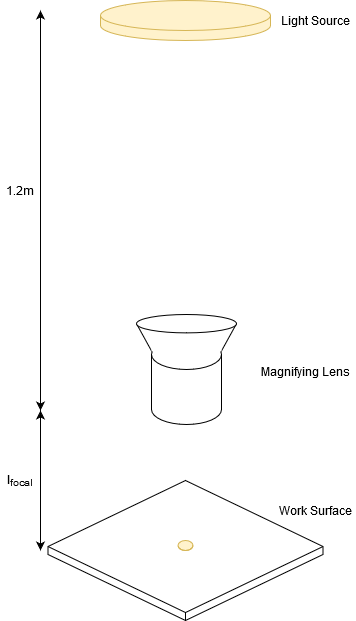
\includegraphics[width=.4\linewidth]{figures/experimentation/focal_length.png}
		\captionof{figure}{Focal Length Experiment Setup}
		\label{fig:focal_length_experiemnt}
\end{figure}

After setting up the experiment, the lens was slowly adjusted along the vertical until the spot formed on the work surface was a minimum. A tape measure was used to find the distance from the work surface to the lens.

\subsubsection{IR Beam Dispersion}

To test the light focusing tube, two power LEDs where used. Initially, a 3W warm white (visible light) power LED was used to confirm the functionality of the system. Following this, the 3W IR power LED was used.

In both cases, the focus system was setup a specific distance from a flat surface. The light was then powered and the edge of the beam spot was marked and the diameter taken. To determine the location of the IR beam spot edge, a video camera in 'night shot' mode was used.

\begin{figure}[H]
	\centering
	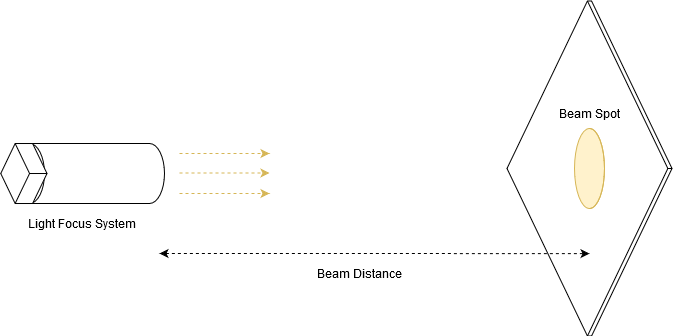
\includegraphics[width=.7\linewidth]{figures/experimentation/beam_spot_experiement.png}
	\captionof{figure}{Light Focus System Experiment Setup}
	\label{fig:focus_system_experiemnt}
\end{figure}

%todo: Give distances for measuredments taken
Figure \ref{fig:focus_system_experiemnt} above shows the experimental setup. The experiment was performed for distances of x, y, z.



%%%%%%%%%%%%%%%%%%%%%%%%%%%%%%%%%%%%%%%%%%%


\subsection{Goertzel Filter Benchmark}

To understand the benefits to be gained from optimization and to understand the effectiveness of the two optimization methods the following experiment were performed to give insight into the effect of increasing the number of samples (N) and optimizing the algorithm by reducing the number of multiplications.

First, the goertzel algorithm as given in listing \ref{lst:goertzel_algorithm} was converted to C and implemented inside the circular buffer's callback functions. This implementation is referred to as the unoptimized algorithm. As a consequence of using a circular buffer with two segments, there are two callback functions. The goertzel implementation inside both callback functions were the same, with the only exception being the location in the buffer from which samples were read.

The timing was measured externally using an oscilloscope, to achieve this, just before the goertzel algorithm began executing an LED was turned on using one of the GPIO pins. This LED was turned off as soon as the algorithm finished calculating the result. Each of the two callback functions used a unique GPIO pin to toggle separate LEDs. Figure \ref{fig:goertzel_optimization_experiemnt} below illustrates the experimental setup in the form of a block diagram.

\begin{figure}[H]
	\centering
	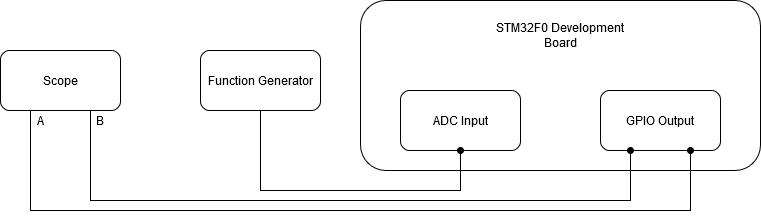
\includegraphics[width=.9\linewidth]{figures/experimentation/goertzel_speed_test_diagram.png}
	\captionof{figure}{Goertzel Optimization Experimental Setup}
	\label{fig:goertzel_optimization_experiemnt}
\end{figure}

A signal generator was used to produce a 36kHz sine waveform with an amplitude of 1V and an offset of 1V. Using a signal generator ensured that a known waveform was present at the input to the goertzel filter, in addition, by using a 36kHz waveform the filter is forced to deal large sample values which gives insight into performance under the most demanding circumstances.

The experiment was broken into iterations, each iteration began by setting N to the desired number of samples, following this the code was compiled and executed on the development board. The signal generator was attached and enabled and the scope probes were attached to the GPIO pins responsible for indicating timing. The scope was then adjusted so that between 20 and 30 pulses could be seen. 

The independent variable N (number of samples to process) was set to 4 for the first iteration and doubled for each consecutive iteration until a value of 64 was reached. These five values of N were chosen because they preserve the ratio given in equation \ref{eqn:k_N_and_fb_fs_ratio} which is a requirement for the optimization to work.

Using the measurement tools built into the Picoscope software the 'high pulse width' for both GPIO pin outputs was measured, along with the duty cycle of those waveforms. The average of all pulses was recorded.

For the purposes of this experiment only the 'high pulse width' of the callback responsible for the first half of the circular buffer being full was necessary to draw conclusions regarding the algorithms performance. The timing for the second half of the buffer being full was used only as a sanity check, both the callback functions should run for the same amount of time as each is executing the same algorithm therefore the average high pulse width for each should be the same.

After the experiment was run for all 5 iterations, the goertzel implementation was modified by removing the unnecessary multiplications (as discussed in section \ref{sec:filter_optimization_design}) and the above experiment repeated following the same method.


%Filter performance experiment:
% - Impact of multiplication in algorithm
% - Impact of N


\subsection{Goertzel Filter Performance}

To evaluate the performance of the goertzel filter the following experiments where performed.

\begin{itemize}
	\item Simulated Frequency Response
	\item Measured Frequency Response
	\item Trigger Conditions
\end{itemize}

\subsubsection{Simulated Frequency Response}
The expected frequency response was determined using the Octave\footnote{Open-source alternative to Matlab} environment. This was achieved by first creating a goertzel filter with the exact same optimized algorithm as the one implemented on the STM32 and a main script to interface with the function. The octave Goertzel function is given in listing \ref{lst:optimized_goertzel_algorithm}. This function is optimized according to the design outlined in section \ref{sec:filter_optimization_design} and the value returned by the function is the magnitude of the DFT coefficient squared.

Following this the interface Octave script was written to find the filter response (see listing \ref{lst:frequency_response_script}). This script generated a range of frequencies in the form of sampled sin waves over the range of 0Hz to 71.7kHz with an interval of 100Hz. To simulate the behaviour of the filter, the test frequencies were scaled, off-set and sampled to match the expected conversion values returned by the ADC. After generating each frequency, the above mentioned octave implementation of the Goertzel filter was called and the computation result stored. An example, 36kHz waveform is given in the appendix, figure \ref{fig:sampled_36khz_sinusoid}.

The frequency response was plotted to provide an insight into the expected performance of the digital filter. The frequency response was tested with sinusoids of amplitude 1V and again with sinusoids of amplitude 500mV.

\subsubsection{Measured Frequency Response}
The next experiment involved testing the Goertzel filter to check that the filter implementation was working as expected. This was done by generating a sinusoid waveform at the input to the ADC and using the serial communication port to transfer the value of the Goertzel filtering result. 

The experimentation was performed on the STM32 development board. This process involved manually configuring the function generator for each individual frequency and then pushing a button on the development board to transfer the most recent filter result.

The first frequency tested was 1kHz, this frequency was incremented by 3kHz per reading until a frequency of 70kHz was reached. The results were processed by Octave to generate a plot and compare the empirical results with the simulated response.


\subsubsection{Trigger Conditions}
%Trigger Frequency vs amplitude | Trigger frequency
To evaluate the high-level functionality of the Goertzel, an experiment was performed to determine the amplitude and frequency boundary pairs which cause the goertzel filter to trigger.

Because no automatic gain control has been implemented in the Goertzel algorithm, there is a minimum signal  amplitude required to trigger the output. This provides insight into this minimum amplitude and how that amplitude changes as the frequency moves away from the centre frequency of 36kHz.

A function generator was connected to the input of the Goertzel filter module and an oscilloscope was connected to the output and also used to monitor the generated waveform. Throughout the experiment the generated sinusoidal waveform was offset by 1V to ensure the input voltage remained positive.

By way of manually adjusting the amplitude, the function generator was used to determine the approximate voltage which would trigger the Goertzel filter for an input frequency of 36kHz. This occurs at around 297mV. For the purposes of experimentation this value was rounded to 300mV.

Starting from 300mV and increasing by increments of 50mV, the amplitude of the generated sinusoid was set. Each time the amplitude was set, the function generator was configured to sweep though all frequencies between 28kHz and 44kHz. The oscilloscope was used to find the frequencies which caused the output of the Goertzel filter to go high. For each amplitude value there are two boundaries, a lower and upper frequency.

These results were then tabulated and plotted using Octave.


\subsection{Carrier Waveform Generation Performance}


\subsection{Power LED Driver Performance}

The LED driver module must be capable of modulating a high-power IR led at a frequency of 36kHz.

To verify that the power LED driver module operates as expected and to evaluate the modules performance, a set of test driving frequencies were injected and the response recorded. Figure \ref{fig:power_led_driver_experiemnet_setup} illustrates the experimental setup.

\begin{figure}[H]
	\centering
	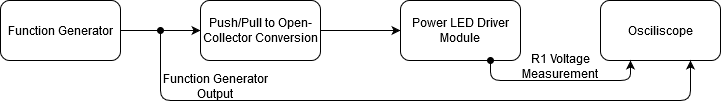
\includegraphics[width=.9\linewidth]{figures/experimentation/power_led_driver_experimental_setup.png}
	\captionof{figure}{Power LED Driver Experimental Setup}
	\label{fig:power_led_driver_experiemnet_setup}
\end{figure}

The test signal is a square wave generated using a function generator. This signal is converted to an open-drain signal before being injected into the driver module. To precisely monitor the LED's state, an oscilloscope was connected across the shunt resistor R1 (see schematic in figure \ref{fig:schematic_power_led_driver}). Monitoring the resistor provides insight into both the state of the LED and the current through the LED. The current through the power LED can be calculated as \(I_{led} = \frac{V_{R1}}{0.7}\).


\subsection{Directivity of detector modules}

To characterise the directivity of the photodiode and phototransistor detector modules, the following experiment was performed.

\begin{figure}[H]
	\centering
	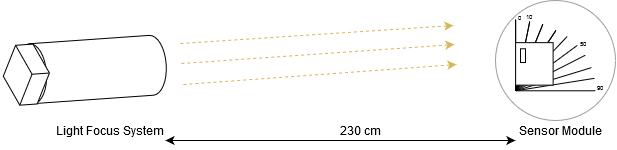
\includegraphics[width=.9\linewidth]{figures/experimentation/beam_angle_of_receiver.png}
	\captionof{figure}{Directivity Experimental Setup}
	\label{fig:directivity_experiement_setup}
\end{figure}

The light focus system was connected to the LED driver module which was modulated at 36kHz by the carrier waveform generator module. The modulated beam was then aimed at the sensor module, placed 230cm away. The output of the detector module was connected to an oscilloscope to trace the output waveform.

The IR beam was positioned off centre so that when the module was adjusted to have an indecent angle of 0\textdegree the output of the sensor module was only just saturating, this ensured the sensitivity could be accurately tracked. Figure \ref{fig:begin_saturation_of_photodiode} in the appendix illustrates the waveform at the output of the photodiode module just after saturation.

Starting with an incidence angle of 0\textdegree, the module was incrementally rotated until a the angle of incidence was equal to 90\textdegree. Each increment involved performing a 10\textdegree rotation and following the rotation the output waveform was exported for processing in Octave.

Octave was used to calculate the RMS\footnote{root mean square} voltages for the recorded output waveforms. In addition, the RMS values were normalized and plotted to provide insight into the detector modules directivity.

The IR receiver module was also tested following the above experimental method, however the output from this module is a logic level indicating the presence of a modulated waveform so it would be non-nonsensical to consider the RMS value, instead the binary state was tracked.

\subsection{Signal Conditioning Performance}

\subsubsection{Anti-alias Filtering}
%todo: experiment here

\subsubsection{Precision Rectification}
%todo: experiement here


\subsection{Tagger MCU Performance}

\subsubsection{Manchester Encoding}

An oscilloscope was connected to the output of the tagger MCU. The Manchester encoded waveform produced was traced and evaluated %todo: evaluteate what?


\subsection{Target MCU Performance}

\subsubsection{Processing Time}

To measure the time it takes the processor to decode Manchester encoded transmissions and determine if it is possible to reduce the dead-time between transmissions, the following experiment was performed. This is achieved by decoding messages with differing lengths in terms of the number of edges in the encoded Manchester sequence.

The receiver algorithm was modified to set a GPIO pin high at the beginning of the Manchester decoding function and reset the pin after the decoding completes. The tagger MCU was then wired directly to the target MCU to remove any external factors that might be introduced by the various intermediate stages.

Three data packets were chosen, based on the corresponding number of edges in the Manchester encoded sequence. The lowest possible number of edges in a valid message is 20 while the highest is 36. The message with the data value 11111 was chosen arbitrarily and contains a number of edges in between the limits.

\begin{table}[H]
	\centering
	\begin{tabular}{ccc}
		\hline
		\textbf{\begin{tabular}[c]{@{}c@{}}15-Bit Data\\ (Decimal)\end{tabular}} & \textbf{\begin{tabular}[c]{@{}c@{}}18-bit Transmission\\ (Hexadecimal)\end{tabular}} & \textbf{Number of Edges} \\ \hline
		10922 & 0x2AAAB & 20 \\ \hline
		11111 & 0x2AD9F & 26 \\ \hline
		32767 & 0x3FFFF & 36 \\ \hline
	\end{tabular}
\end{table}

%todo: complete this experiment description by adding timeout period
An oscilloscope was used to trace the incoming Manchester waveform and the state of the GPIO being toggled before and after the processing function. This allowed measurement of both the length of the computation time and the length of the timeout period.





\subsection{System Range}

To determine the range of the laser tag system, the system was setup on a large field and the distance between the tagger and target modules gradually increased until errors in the incoming transmission began to occur.

The maximum distance was defined to be the distant at which practically all transmissions were received successfully, but occasionally a bit error would occur. This distance was measured using a tape measure.

The three different detector modules were tested in turn and the experiment was performed both at night and during the day. This allowed a comparison between the range and effects of ambient sunlight of the three detectors.

The Picoscope oscilloscope was used to capture the waveform at the input and output of the goertzel filter for inspection.